\entry{Semana del 12/05/2025}
\section{Lunes 12/05/2025}
Hoy fuimos a tratar de probar el sensor con el Lock-in SR830 de Laboratorio 4/5, que se supone debería ser capaz de medir flotante. 

También ya recubrimos la punta del cable de cobre con el esmalte aislante cerca de la ventana y lo montamos en una estructura de perfiles que montó Pablo para sumergirlo en una pecera llena de agua destilada, después de dejarlo secar unos 10 minutos. Apoyarlo solo sobre cajas que fue lo primero que probamos no funcionó ya que el centro de masa estaba muy por delante y hacía que rote y no se quede derecho. 

\begin{figure}[!ht]
	\centering
	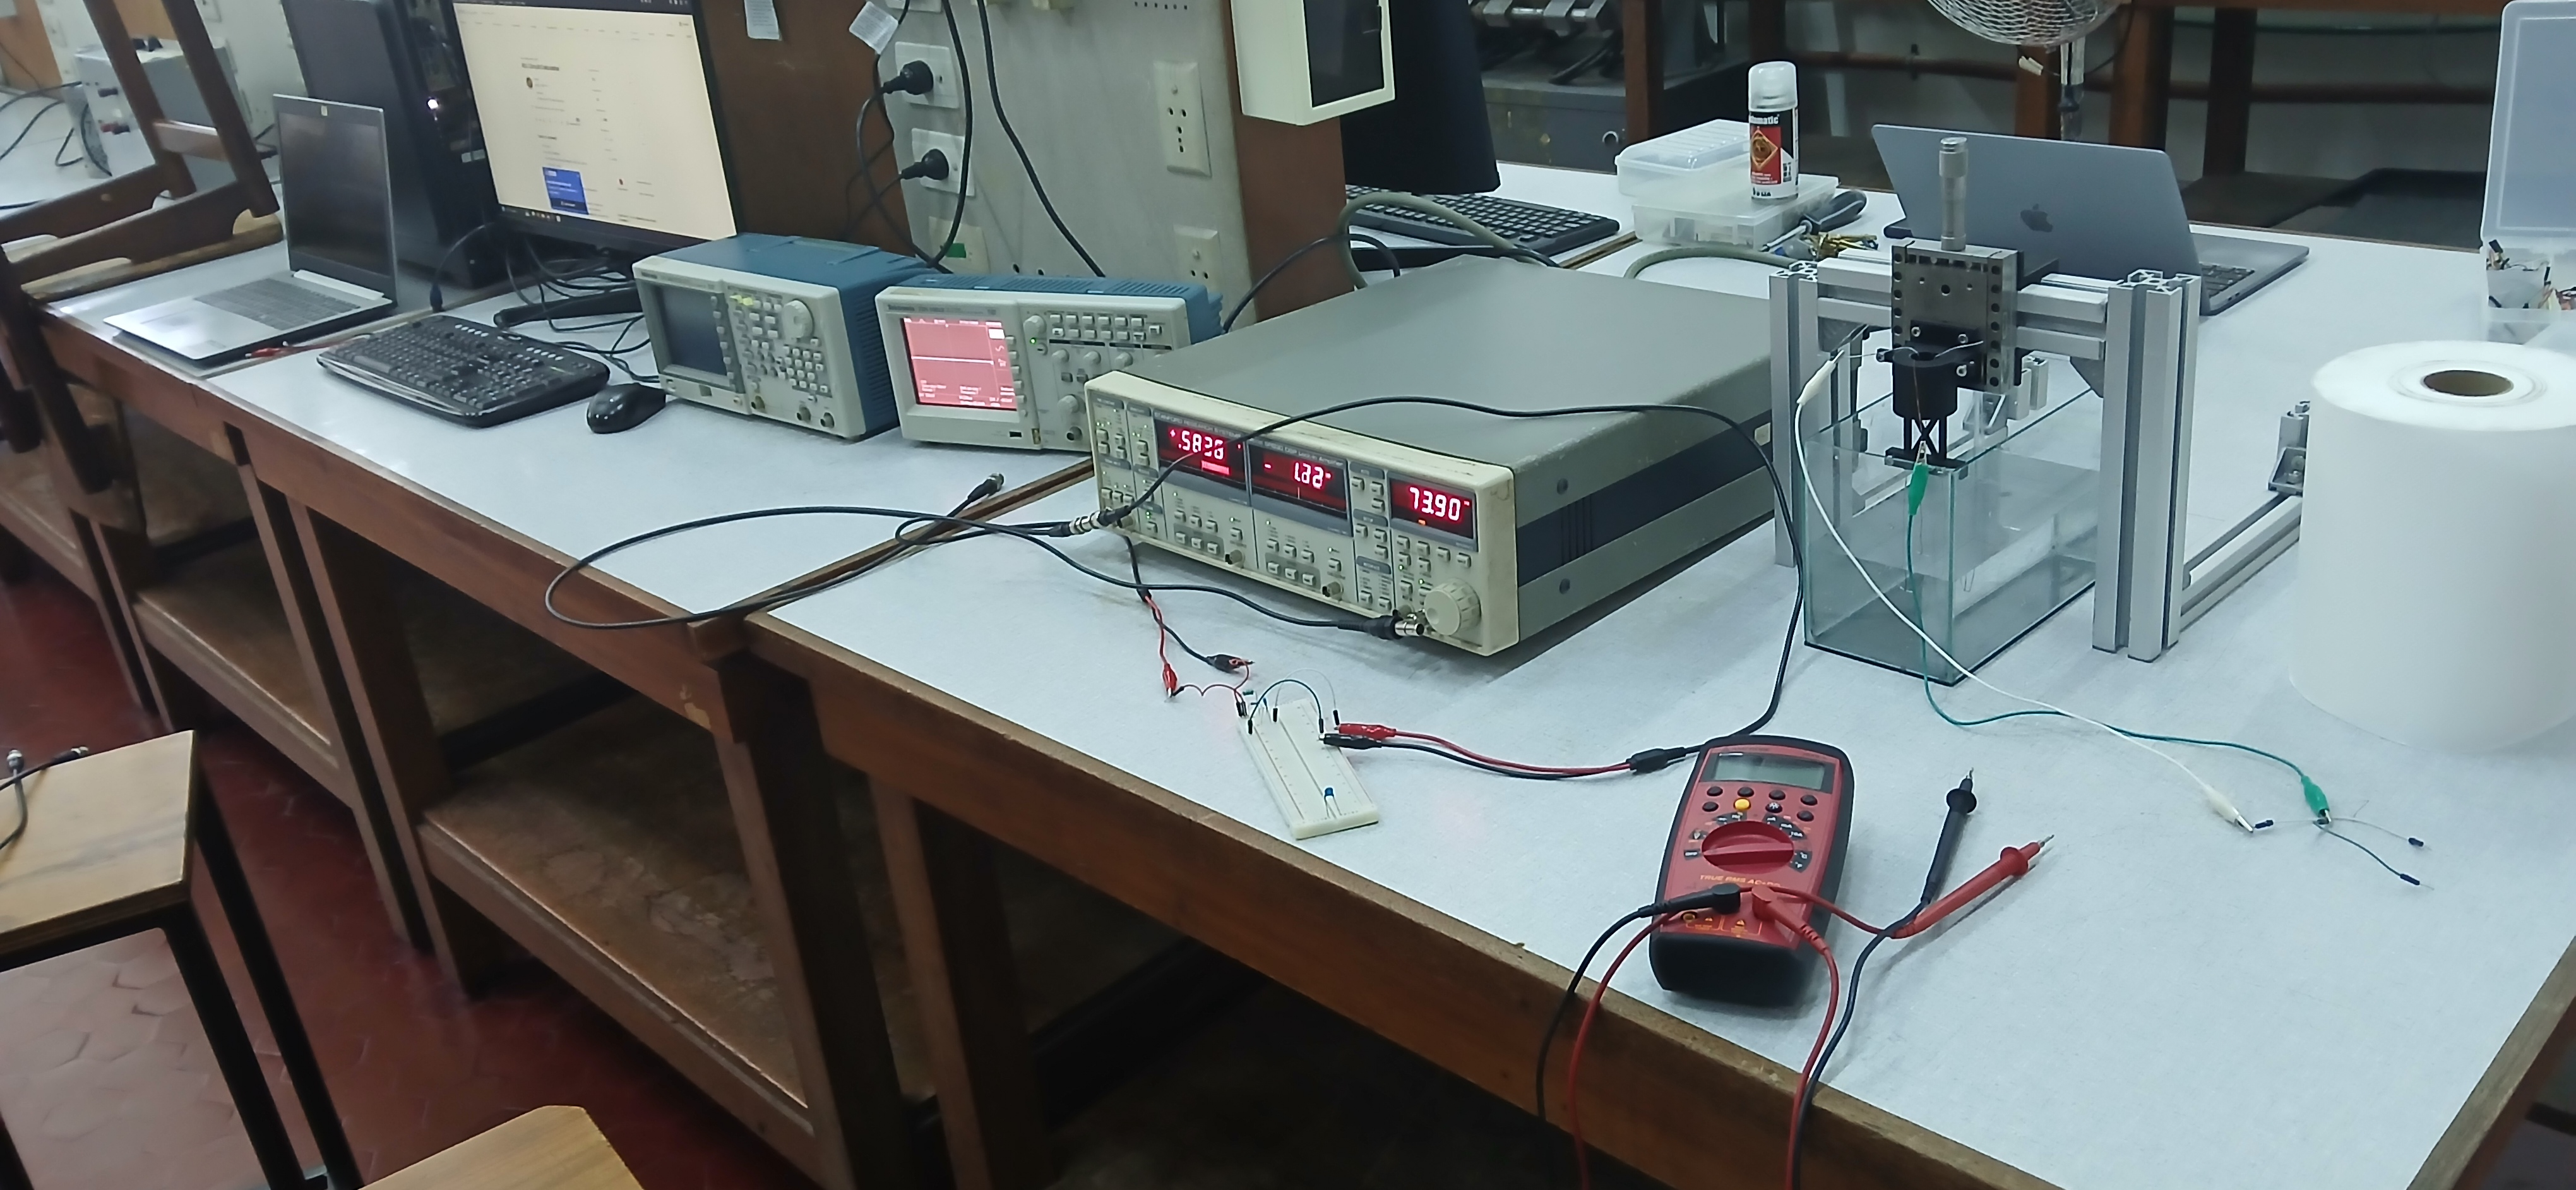
\includegraphics[width=0.7\linewidth]{Figures/12_05_2025/20250512_113406.jpg}
	\caption{Setup para usar el sensor y el Lockin}
	\label{fig:foto_12_05_2025}
\end{figure}

Conectamos todo, sin embargo el Lockin estaba teniendo mucho ruido. Pasamos a conectar directamente la salida del generador de funciones a la entrada del lock-in y a la referencia externa, sin embargo seguía fallando ya que no estaban en fase. La amplitud estaba bien, ya que era de 2 Vpp del generador y daba 0.71 que es la RMS, que se relacionan:

\begin{equation}
	V_{pp} = 2\sqrt{2} V_{rms} % () 
\end{equation} 

Pasamos a usar la referencia interna y funcionaba bien tanto la amplitud (que ahora era RMS la marcada por el equipo) como la fase de aproximadamente 0°. Para esto usamos un tiempo de integración de aproximadamente 1 ms, entrada A para que no salte el fusible. % ,, 

Después probamos conectar el RLC con el sensor pero estaba marcando cosas raras. Ahí con el oscilosocopio nos dimos cuenta de que el cable BNC estaba roto y lo cambiamos. Después igualmente siguió dando cosas raras así que desconectamos el sensor y nos centramos en el RLC. Éste ahora tenía C=560 pFcon una frecuencia de resonancia teórica de 67 kHz aproximadamente. Conectado Tierra con Tierra en unos 73 kHz daba máximo de amplitud y fase casi de 0° pero al cambiar de lugar la resistencia y el capacitor dejaba de funcionar (siempre midiendo sobre la resistencia).  Importante también que no se toquen las cabezas de las pinzas para que no haga corto el circuito. % n ´pe  

Después dejamos fijos los componentes y dimos vuelta el orden de los cables que medían sobre la resistencia. Cuando estaba el negro con el negro funcionaba bien pero al rotarlos no, incluso cuando estaba en flotante. 

Probando continuidad no parecen estar conectadas las cabezas de la salida de la referencia interna con la de la entrada de voltaje (sí al poner negro con negro). 

Cambiamos las posiciones de los componentes en la Protoboard para verificar que no fuese eso pero no pareció cambiar el comportamiento. Al rotar los cables de lugar pasaba de unos 2° a unos 77° que no es el salto en 90° esperado por el cambio del signo al medir el votaje en la otra dirección. % ¬ % & % ¬ % | % ¬ 

Ya después de eso cerca de las 12:00 decidimos guardar todo y volver al Laboratorio ya que el comportamiento no era el esperado. 

Incluso manteniendo el sentido de los cables al cambiar de lugar la capacitancia y la resistencia daban cuatro valores distintos, dos por cada posición (cables normales e invertidos). 

Probablemente lo mejor sea usar una placa de adquisición para no preocuparnos por el tema de la Tierra y luego procesar a posteriori usando el filtro pasa bajos. 

\begin{figure}[!ht]
	\centering
	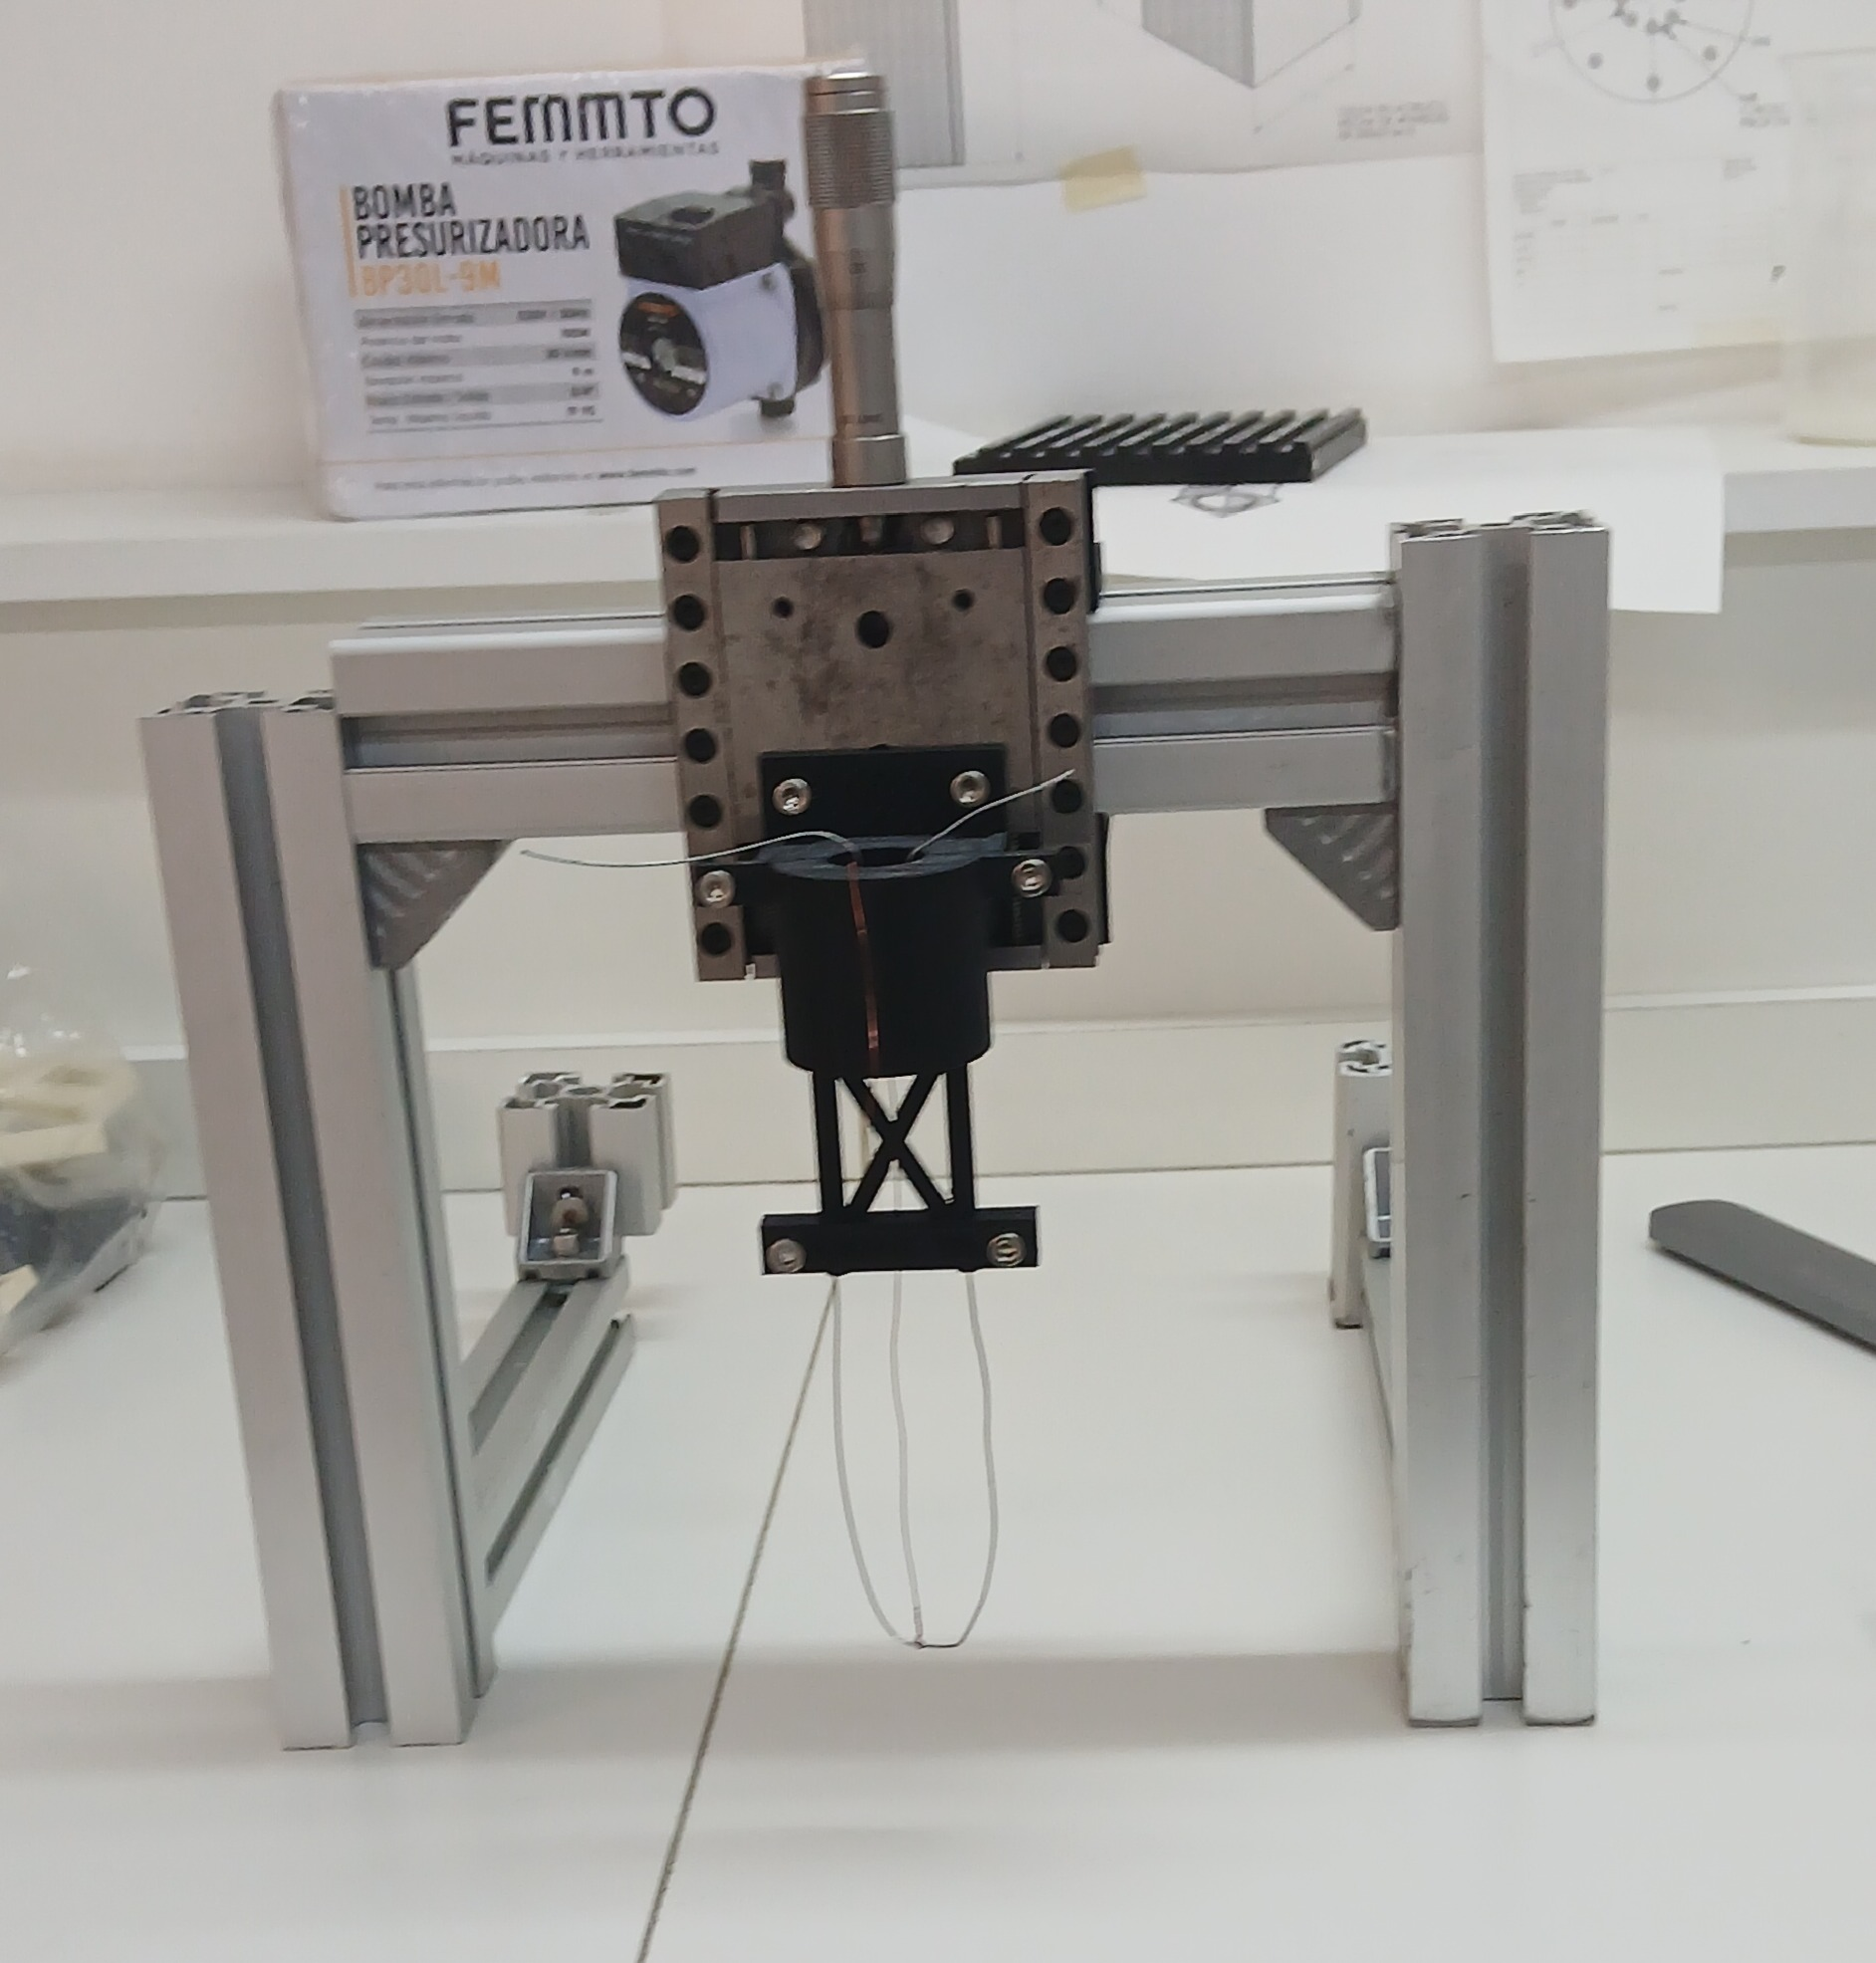
\includegraphics[width=0.7\linewidth]{Figures/12_05_2025/20250512_140434.JPG}
	\caption{Sensor completo montado ya sobre el soporte.}
	\label{fig:foto_sensor_completo_12_05_2025}
\end{figure}